
\chapter{Experimental Results}
\label{chap:validation}
This chapter presents the evaluation of the key subsystems developed for the GolfBot project. The performance of each component was assessed through a series of quantitative and qualitative tests designed to validate its effectiveness in fulfilling its designated role.

\section{Computer Vision System Evaluation}
\label{sec:cv_evaluation}
The performance of the computer vision system was evaluated in two stages. First, a quantitative analysis of the trained YOLOv11-seg model was conducted using the hold-out test dataset to assess its detection accuracy. Second, a qualitative real-world test was performed to observe the model's robustness in a live operational scenario.

\subsection{Divot Detection Accuracy}
\label{ssec:cv_accuracy}

The accuracy of the trained YOLOv11-seg model was evaluated using standard metrics in the field of object detection. The primary metrics used are Precision (the accuracy of the positive predictions) and Recall (the ability of the model to find all relevant instances).

The relationship between these two metrics is captured by the Precision-Recall (P-R) curve, shown in Figure \ref{fig:accuracy_metrics}a. A model whose curve is close to the top-right corner maintains high precision even as it finds a high percentage of true objects (high recall). The area under this curve is summarized by the Mean Average Precision (mAP) score, which is the single most important metric for evaluating object detector performance. The model achieved \texttt{mAP@0.5} score of 0.954 across all classes, indicating a high level of accuracy on the test dataset.

To better understand the model's classification performance, a normalized confusion matrix was also generated, as shown in Figure \ref{fig:accuracy_metrics}b. This matrix details the classification accuracy for each class, showing that the model is highly effective at its primary task:
\begin{itemize}
    \item It correctly identified true \texttt{divot} instances 98\% of the time.
    \item It correctly identified true \texttt{fixed\_divot} instances 90\% of the time.
    \item The most common error was misclassifying a \texttt{fixed\_divot} as background (10\% of the time), which is an acceptable failure mode as it avoids attempting to repair an already fixed divot.
\end{itemize}

\begin{figure}[h!]
    \centering
    % === SUBFIGURE 1: P-R CURVE ===
    \begin{subfigure}[b]{0.49\textwidth}
        \centering
        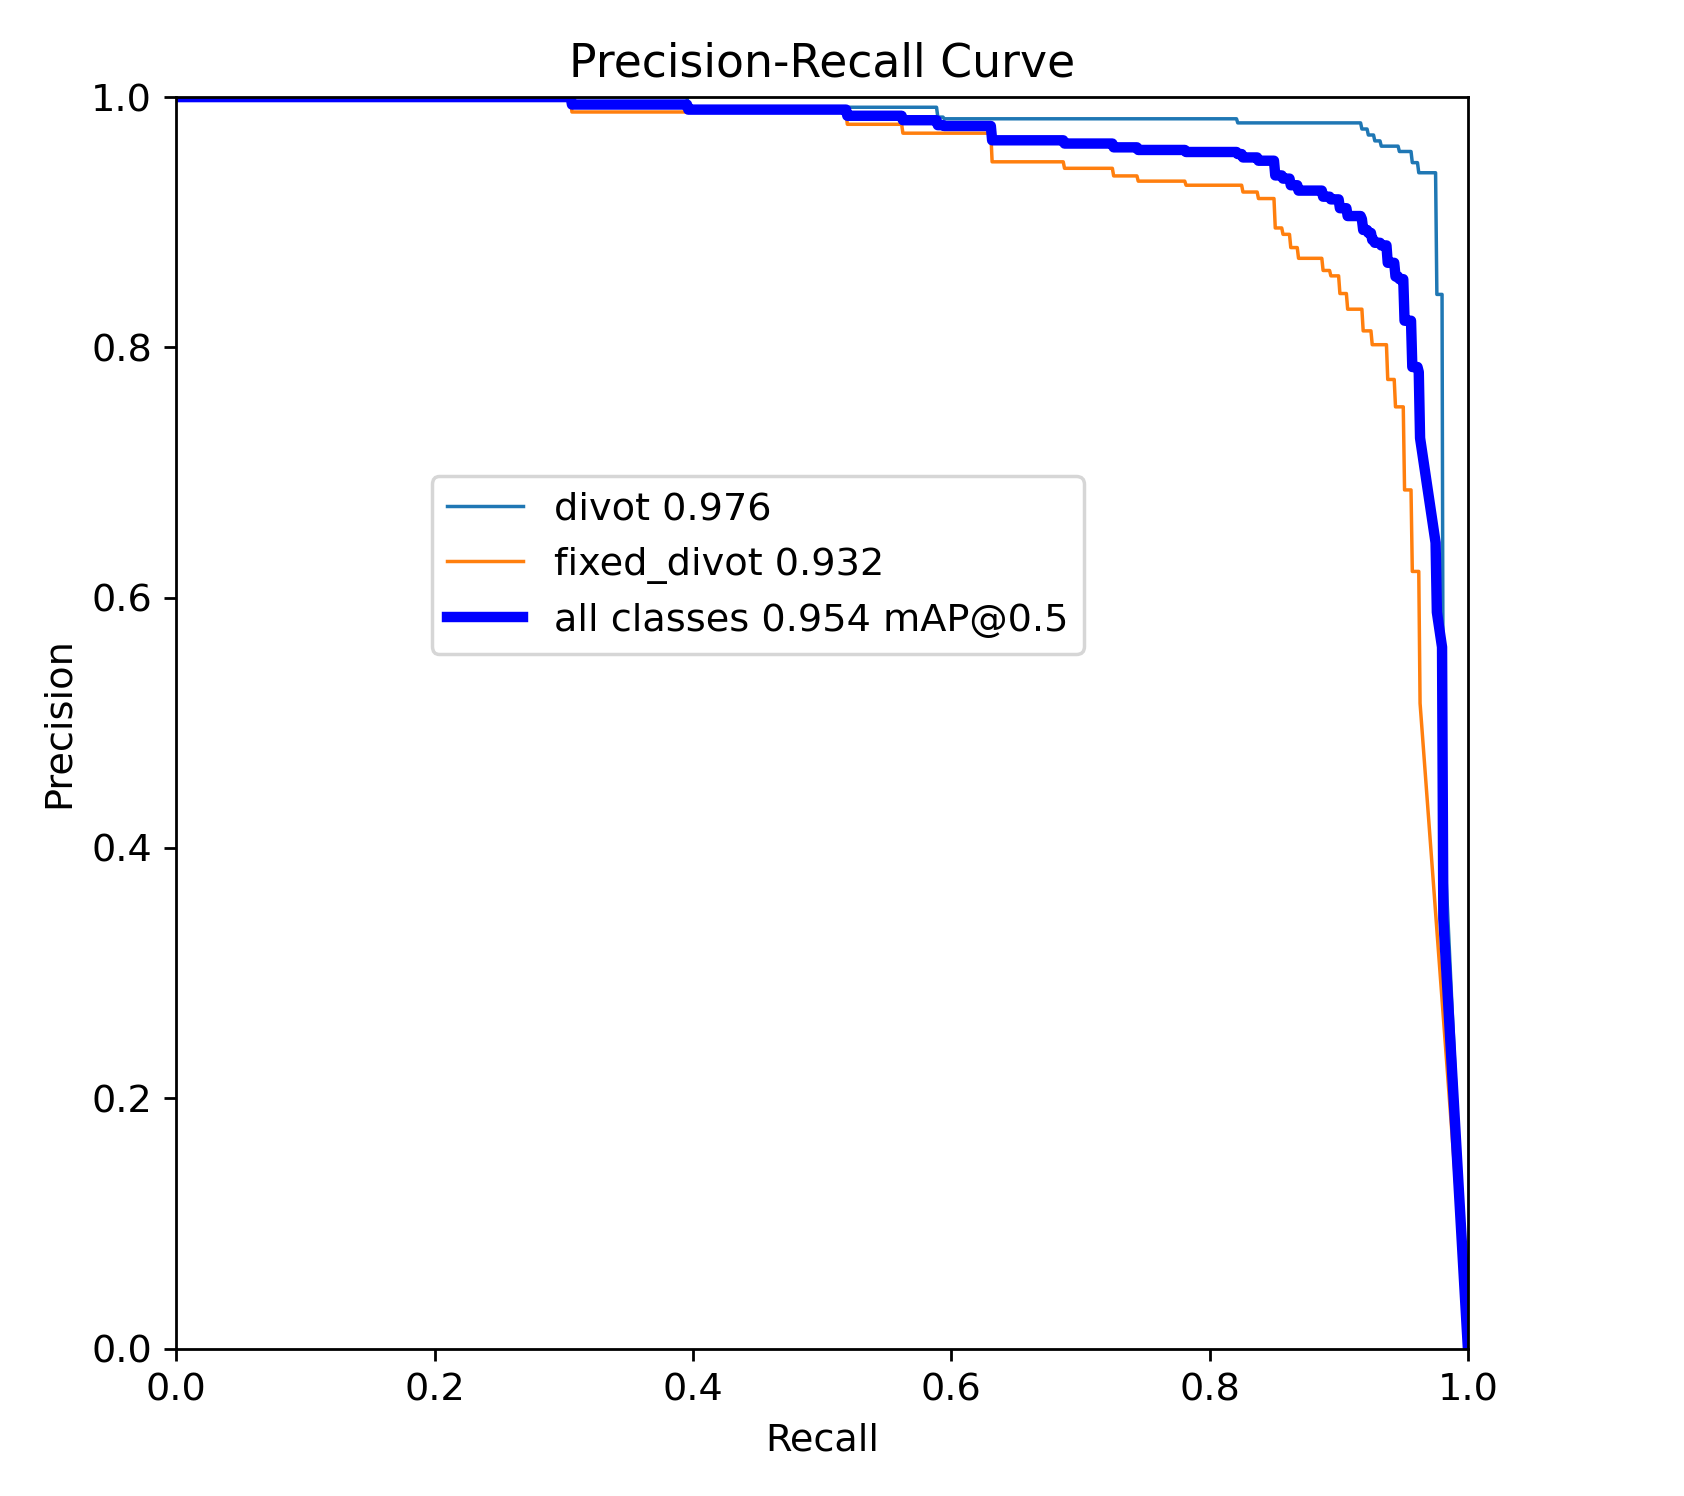
\includegraphics[width=\textwidth]{figures/precision_recall_curve.png}
        \caption{Precision-Recall (P-R) Curve.}
        \label{fig:pr_curve_sub}
    \end{subfigure}
    \hfill 
    % === SUBFIGURE 2: CONFUSION MATRIX ===
    \begin{subfigure}[b]{0.49\textwidth}
        \centering
        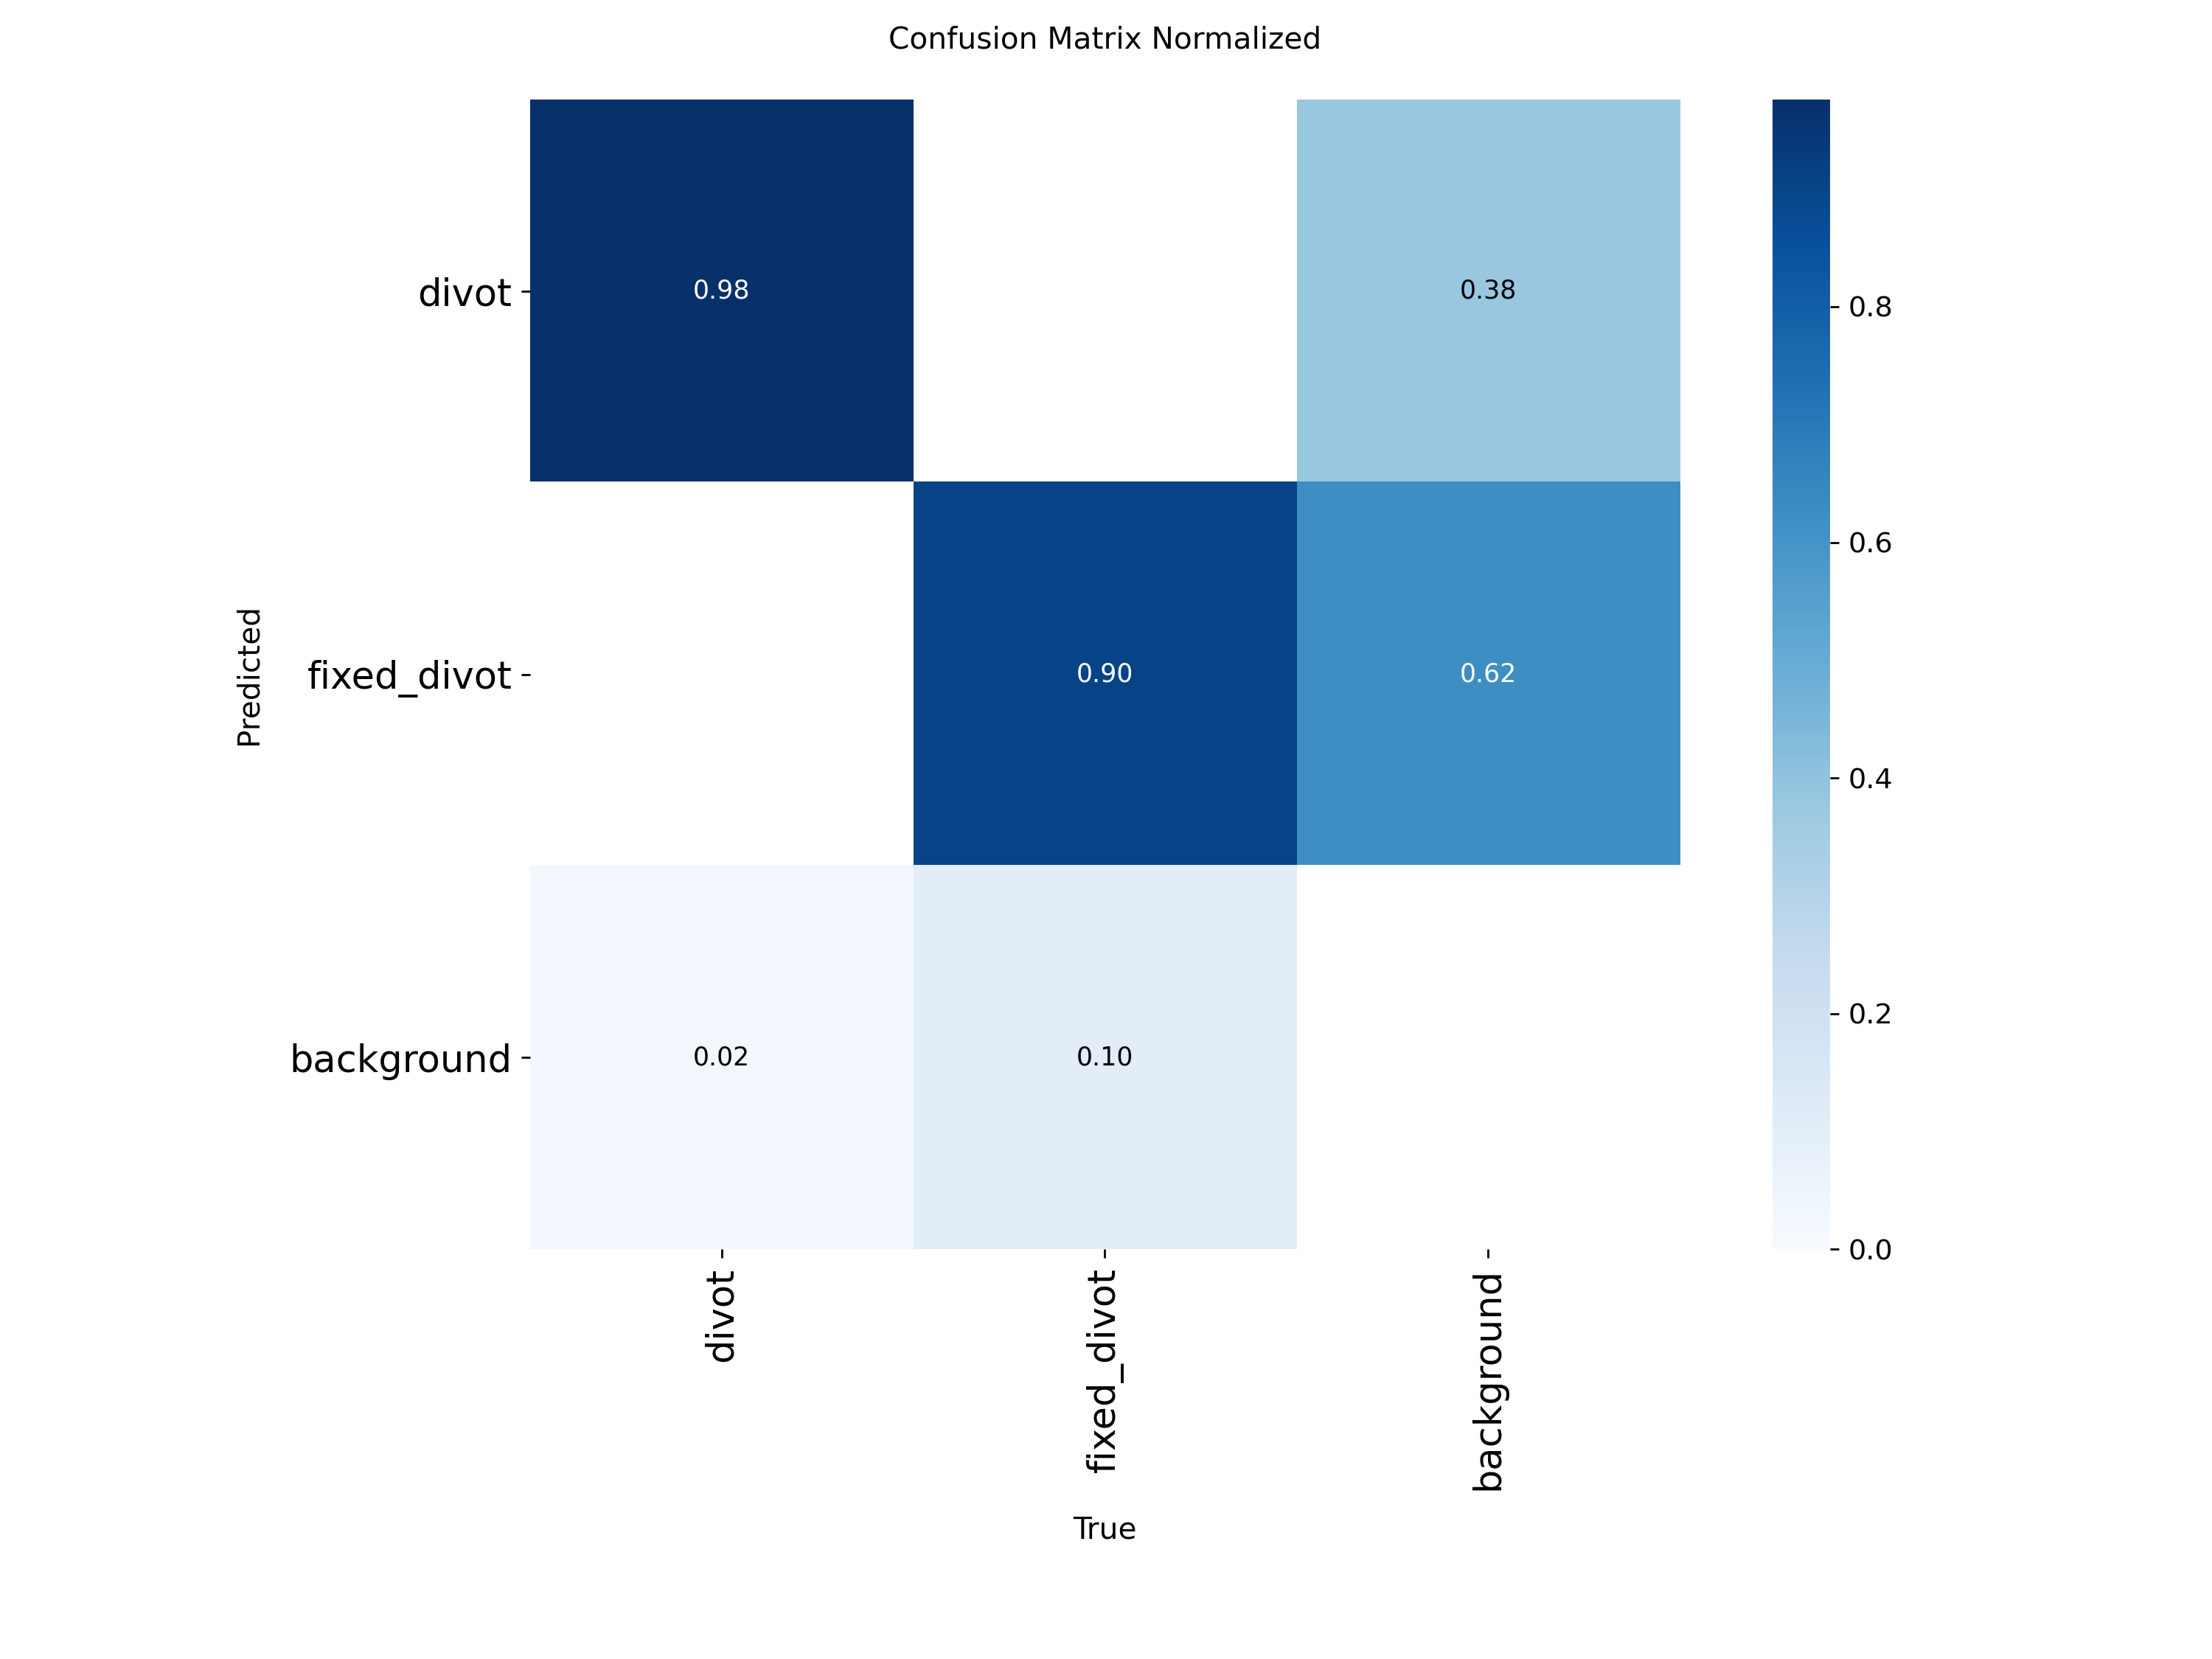
\includegraphics[width=\textwidth]{figures/confusion_matrix_normalized.png}
        \caption{Normalized Confusion Matrix.}
        \label{fig:cm_sub}
    \end{subfigure}
    
    \caption[Key Performance Metrics: P-R Curve and Confusion Matrix.] 
    {Quantitative evaluation of the model's accuracy. The P-R curve (a) visualizes the model's mAP score of 0.954, while the confusion matrix (b) details the specific classification performance for each class.}
    \label{fig:accuracy_metrics}
\end{figure}

In addition to these quantitative metrics, a qualitative comparison of the model's performance on the unseen validation set is provided in Figure \ref{fig:validation_comparison}. The figure directly compares the ground truth labels (a) with the model's predictions (b) on the same set of images. The high degree of visual similarity between the two provides strong qualitative evidence of the model's effectiveness. The model successfully identifies a variety of divot shapes and sizes under different lighting conditions.

\begin{figure}[h!]
    \centering
    \begin{subfigure}[b]{0.49\textwidth}
        \centering
        \includegraphics[width=\textwidth]{figures/val_batch1_labels.png}
        \caption{Ground truth labels}
        \label{fig:val_labels}
    \end{subfigure}
    \hfill 
    \begin{subfigure}[b]{0.49\textwidth}
        \centering
        \includegraphics[width=\textwidth]{figures/val_batch1_pred.png}
        \caption{Model's predictions}
        \label{fig:val_preds}
    \end{subfigure}
    \caption{Visual comparison of ground truth labels (a) and the model's predictions (b) on a sample batch of images from the unseen validation set.}
    \label{fig:validation_comparison}
\end{figure}

These quantitative and qualitative results confirm that the model is well-trained and highly capable of distinguishing between divots, fixed divots, and the background environment. For a more detailed analysis, a full set of performance graphs—including the F1-Confidence curve, the complete training and validation history, and segmentation accuracy curves—are provided in Appendix \ref{sec:appendix_model_graphs}.

\subsection{Real-World Performance}
\label{ssec:cv_real_world}

While quantitative metrics validate the model's performance on a static dataset, a qualitative test was conducted to assess its performance in a dynamic, real-world scenario. A full on-course test with the integrated robot was not feasible due to the mechanical limitations of the base platform's wheels.

Instead, a live test of the computer vision system was conducted directly on a golf course. The Intel RealSense camera was connected to a laptop running the exact same \texttt{divot\_detector} ROS 2 node used on the robot. The test involved capturing a live video feed while walking slowly across different sections of the fairway, allowing for real-time inference and evaluation of the model's robustness to novel data.

The results highlight how environmental factors influence the model's performance. As demonstrated in Figure \ref{fig:real_world_good}, on sections of the course with uniform, healthy green turf, the model performed exceptionally well, successfully identifying an estimated 98\% of both \texttt{divot} and \texttt{fixed\_divot} classes. The clear visual contrast in these ideal conditions allowed the model to generalize effectively.

In contrast, as shown in Figure \ref{fig:real_world_bad}, on sections with less uniform turf containing patches of discoloration or different grass types, the model's performance was slightly degraded. It failed to identify some divots that were less distinct from the varied background. Furthermore, it was observed that variable lighting conditions, such as harsh shadows or direct sunlight, could also lead to inconsistent detections.

Overall, this qualitative test confirms that the core computer vision pipeline is fundamentally viable. It also clearly identifies that further training with a more diverse dataset, incorporating these challenging turf and lighting variations, is the key next step to achieving full real-world robustness.

\begin{figure}[h!]
    \centering
    % === FIRST SUB-FIGURE: ORIGINAL IMAGE ===
    \begin{subfigure}[b]{0.49\textwidth}
        \centering
        \includegraphics[width=\textwidth]{figures/perfect.png} 
        \caption{Original image on uniform turf.}
        \label{fig:good_original}
    \end{subfigure}
    \hfill % Pushes the two sub-figures apart
    % === SECOND SUB-FIGURE: PREDICTION IMAGE ===
    \begin{subfigure}[b]{0.49\textwidth}
        \centering
        \includegraphics[width=\textwidth]{figures/perfect_processed.png} 
        \caption{Model's successful predictions.}
        \label{fig:good_prediction}
    \end{subfigure}
    % === MAIN CAPTION FOR THIS FIGURE ===
    \caption[High-performance example of divot detection.]
    {An example of the model's high performance on uniform turf, showing the original image (a) and the corresponding, highly accurate predictions (b).}
    \label{fig:real_world_good}

\end{figure}

\begin{figure}[h!]
    \centering
    % === FIRST SUB-FIGURE: ORIGINAL IMAGE ===
    \begin{subfigure}[b]{0.49\textwidth}
        \centering
        \includegraphics[width=\textwidth]{figures/not_perfect.png} 
        \caption{Original image on varied turf.}
        \label{fig:bad_original}
    \end{subfigure}
    \hfill 
    % === SECOND SUB-FIGURE: PREDICTION IMAGE ===
    \begin{subfigure}[b]{0.49\textwidth}
        \centering
        \includegraphics[width=\textwidth]{figures/not_perfect_processed.png} 
        \caption{Model's predictions with a missed detection.}
        \label{fig:bad_prediction}
    \end{subfigure}
    % === MAIN CAPTION FOR THIS FIGURE ===
    \caption[Limitations of divot detection on varied turf.] 
    {An example showing the model's limitations on less uniform turf. The model correctly identifies most divots but misses one that is less distinct from the background.}
    \label{fig:real_world_bad}
\end{figure}

\section{Depth and Volume Estimation Accuracy}
\label{sec:volume_evaluation}
A key objective of the computer vision system is not just to detect divots, but also to estimate their physical size to determine the required amount of repair material. To validate the accuracy of the depth-based measurement algorithm, a controlled experiment was conducted.

\textbf{Experimental Setup.}
As a real-world divot has an irregular shape and depth, a standardized target was used for this test. A shallow, rectangular box with ground-truth dimensions of 11 cm x 5 cm x 2 cm was placed on a flat surface. The Intel RealSense camera was mounted on a tripod at a fixed height, pointing directly down at the target, as shown in Figure \ref{fig:volume_test_setup}. A custom Python script (\texttt{divot\_depth\_seg\_mask\_est.py}) was developed to perform the measurement. This script uses HSV color thresholding to segment the dark interior of the box (simulating a divot) from the light-colored "ground" plane around it.

\begin{figure}[h!]
    \centering
    \begin{subfigure}[b]{\textwidth}
        \centering
        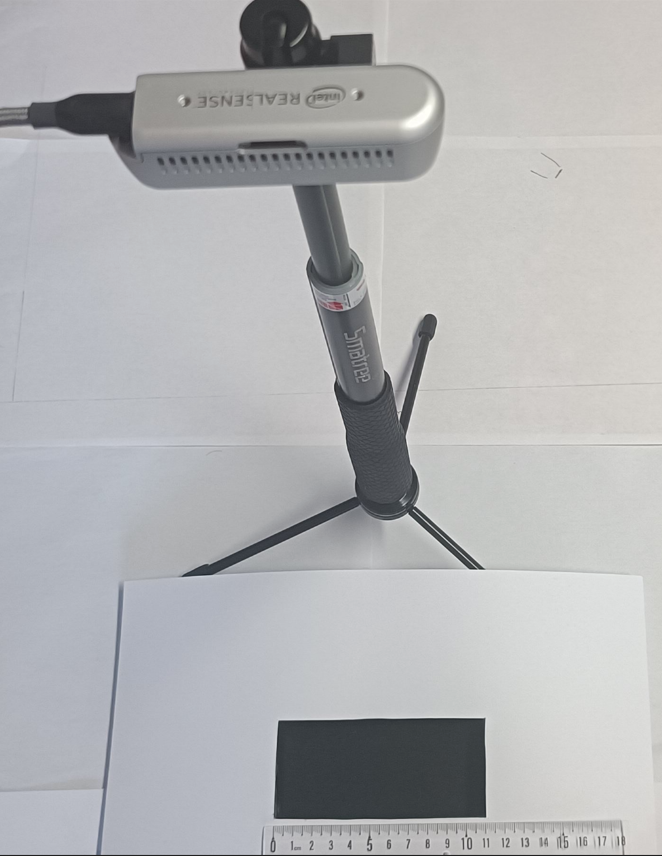
\includegraphics[width=0.6\linewidth]{figures/volume_test_setup.png}
        \caption{Experimental setup showing the camera positioned over a target of known dimensions.}
        \label{fig:volume_test_setup_img}
    \end{subfigure}
    
    \vspace{0.5cm} % Add some vertical space between the setup and the results

    \begin{subfigure}[b]{0.49\textwidth}
        \centering
        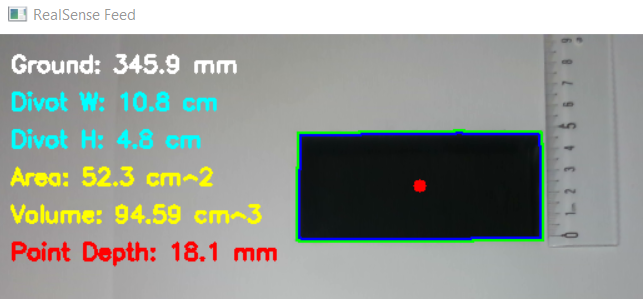
\includegraphics[width=\linewidth]{figures/volume_test_result_5_fix.png}
        \caption{Result from Trial 1.}
        \label{fig:volume_test_result_1}
    \end{subfigure}
    \hfill
    \begin{subfigure}[b]{0.49\textwidth}
        \centering
        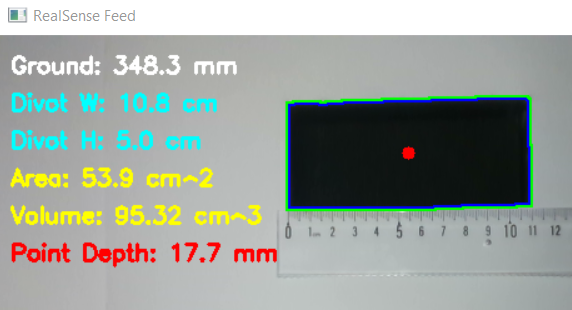
\includegraphics[width=\linewidth]{figures/volume_test_result_11_fix.png}
        \caption{Result from Trial 2.}
        \label{fig:volume_test_result_2}
    \end{subfigure}
    \caption{The controlled experiment to validate the volume estimation algorithm. The setup (a) and two sample results (b, c) showing the system's calculated dimensions and volume.}
    \label{fig:volume_test_setup}
\end{figure}

\textbf{Measurement Algorithm.}
The script calculates the volume using a pixel-by-pixel integration method. It first determines the average depth of the surrounding ground plane. Then, for each pixel inside the segmented divot mask, it calculates the depth difference relative to this ground plane. The real-world area of each pixel is estimated using the camera's intrinsic parameters. The total volume is the sum of the volume of all these tiny pixel columns.

\textbf{Results.}
The system consistently produced measurements with a high degree of accuracy. 
Across multiple trials, the calculated dimensions were within ±2 mm of the 11 cm x 5 cm ground truth. 
The calculated volume averaged between 95–100 cm³, compared to the ground-truth volume of 110 cm³ (11 x 5 x 2), corresponding to an error in the range of 9–14\%. This result demonstrates that the depth perception and measurement algorithm is reliable and capable of producing consistent volume estimates. The integration of this algorithm with the YOLO-based detector to measure irregular divot shapes is a key area for future work, and these calculations will be further refined in future iterations of the system.




\subsection{Navigation System Evaluation}
\label{ssec:nav_evaluation}

The primary objective of the navigation system evaluation was to verify two key aspects: first, the successful integration of the ArduSimple RTK-GPS module into the ROS 2 framework, and second, the real-world positional accuracy of the system. All tests were conducted outdoors with a clear sky view to ensure optimal satellite reception.

\subsubsection{System Integration and Fix Quality}
To confirm the system's integration and fix quality, the robot was powered on and the output of the GPS driver node was monitored in real-time. As shown in Figure \ref{fig:gps_integration}, the system successfully achieved and maintained a high-quality RTK Fixed status (often denoted as `status: 2` in ROS 2 NavSatFix messages). This is the highest level of precision for an RTK system, providing a reported accuracy of approximately 1.4 cm, which is well within the requirements for precise divot repair. The data was successfully published to ROS 2 topics and visualized in the GUI, confirming correct software integration.

\begin{figure}[h!]
    \centering
    % SUBFIGURE 1: GUI
    \begin{subfigure}[b]{0.4\textwidth}
        \centering
        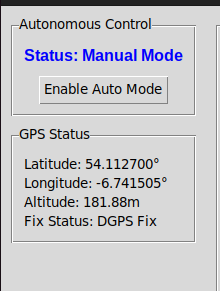
\includegraphics[width=\textwidth]{figures/gui_gps_status.png} % Replace with your GUI screenshot filename
        \caption{GUI displaying GPS status.}
        \label{fig:gui_gps_sub}
    \end{subfigure}
    \hfill % Pushes the subfigures apart
    % SUBFIGURE 2: TERMINAL
    \begin{subfigure}[b]{0.58\textwidth}
        \centering
        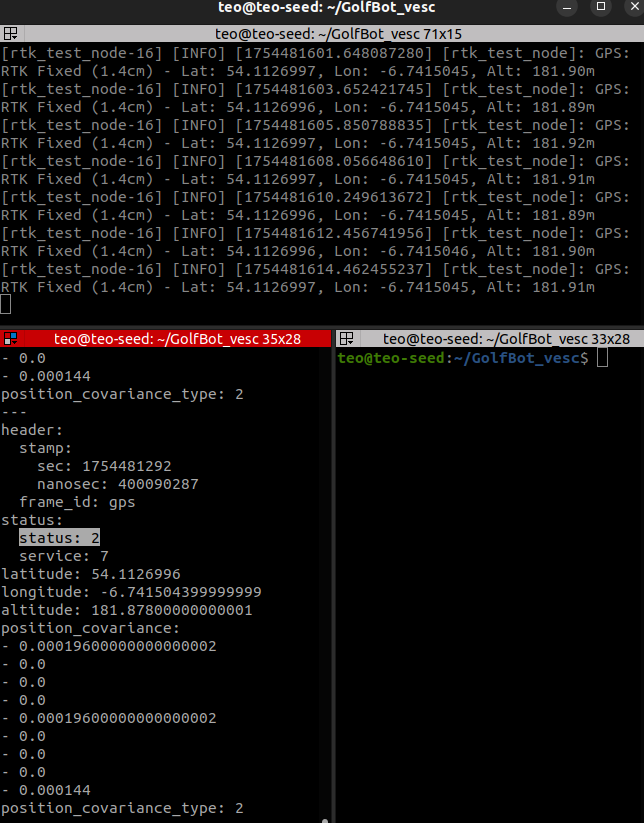
\includegraphics[width=\textwidth]{figures/rtk_terminal_output.png} % Replace with your terminal screenshot
        \caption{Terminal output confirming RTK Fixed status.}
        \label{fig:rtk_terminal_sub}
    \end{subfigure}
    % MAIN CAPTION
    \caption[RTK-GPS System Integration and Fix Status.]
    {Confirmation of the RTK-GPS system's successful integration. The GUI (a) displays a live "DGPS Fix", while the ROS 2 node output (b) confirms the highest-precision "RTK Fixed" status with 1.4 cm accuracy.}
    \label{fig:gps_integration}
\end{figure}

\subsubsection{Positional Accuracy Test}
A practical test was designed to measure the system's translational accuracy. The robot was placed at a designated starting point on a flat surface, and its initial RTK coordinates were recorded. A measuring tape was used to mark a point exactly 1.0 meter forward from the robot's reference point, as shown in Figure \ref{fig:1m_test}. The robot was then manually driven forward until its live GPS coordinates reported a 1.0-meter displacement from the starting position.

The results were highly positive. The robot's final physical position was visually confirmed to be within 2 cm of the 1-meter mark on the tape measure. This practical test validates that the RTK-GPS system provides true centimeter-level accuracy, enabling the robot to reliably track its position and movement for precise, targeted operations.

\begin{figure}[h!]
    \centering
    % SUBFIGURE 1: START POSITION
    \begin{subfigure}[b]{0.49\textwidth}
        \centering
        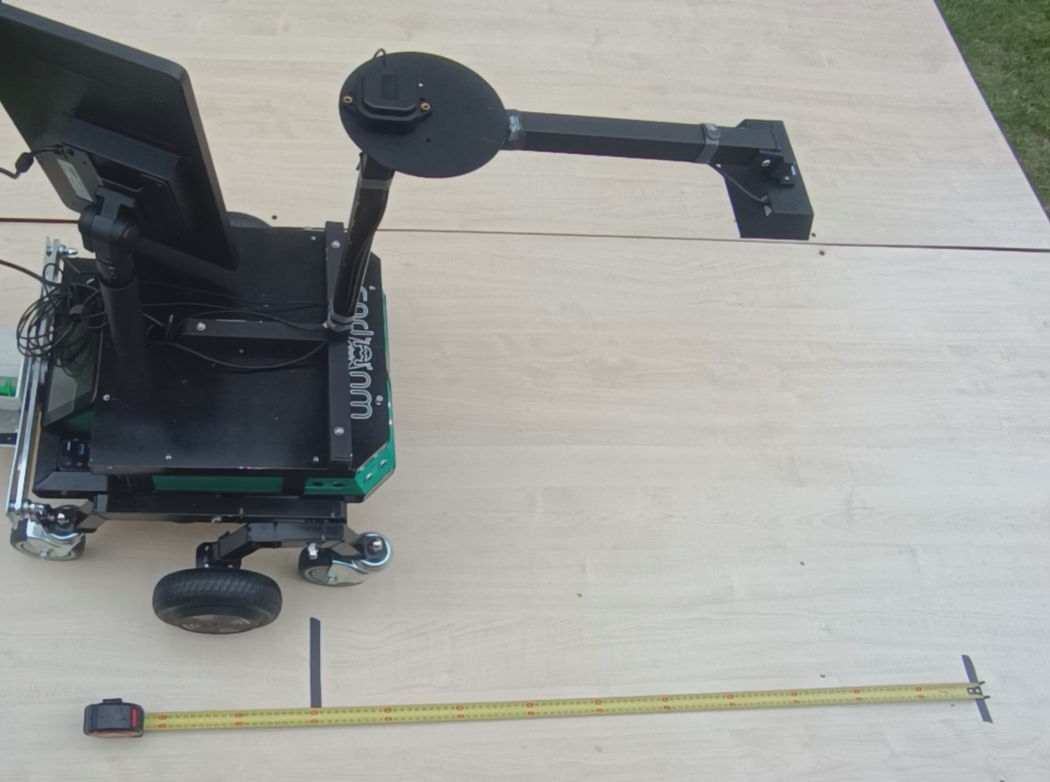
\includegraphics[width=\textwidth]{figures/rtk_test_1.PNG} 
        \caption{Robot at the initial 0m starting point.}
        \label{fig:start_pos_sub}
    \end{subfigure}
    \hfill 
    % SUBFIGURE 2: END POSITION
    \begin{subfigure}[b]{0.49\textwidth}
        \centering
        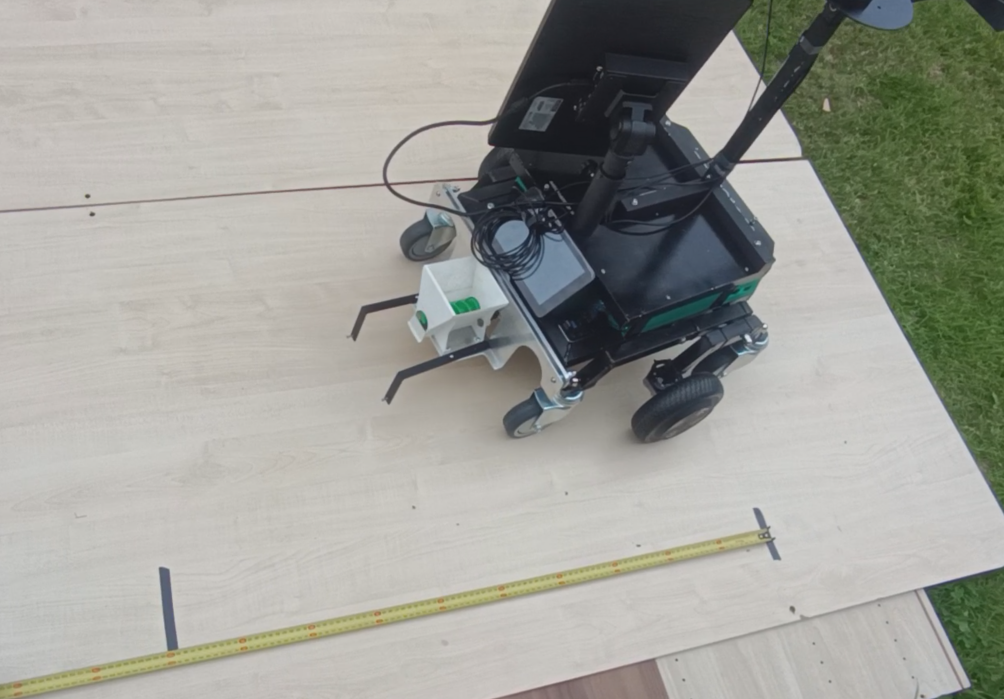
\includegraphics[width=\textwidth]{figures/rtk_test_2.PNG} 
        \caption{Robot at the final 1m target point.}
        \label{fig:end_pos_sub}
    \end{subfigure}
    % MAIN CAPTION
    \caption[One-Meter Positional Accuracy Test.]
    {The physical setup for the 1.0-meter displacement test. The robot was commanded to move from the start position (a) to the target mark (b), with its final position validated against the measuring tape.}
    \label{fig:1m_test}
\end{figure}


\section{Mechanical Dispenser Evaluation}
\label{sec:dispenser_evaluation}
The final component to be evaluated was the mechanical dispenser, which is responsible for the physical act of repair. The evaluation focused on validating the consistency, repeatability, and controllability of its output, which are critical for implementing a 'volume-matched' repair strategy.

\subsection{Dispensing Consistency and Flow Rate}
To quantitatively measure the dispenser's performance, a series of timed flow rate tests were conducted. The motor was run for intervals of 5, 10, 15, and 20 seconds, with three trials performed for each interval to ensure repeatability. The dispensed material was collected and its volume was measured using a measuring cup, as illustrated in the experimental setup shown in Figure \ref{fig:dispenser_test}. For these tests, the stepper motor was configured with a maximum speed of 2000 steps/second and an acceleration of 2000 steps/second², providing a consistent operational baseline.

\begin{figure}[h!]
    \centering
    \begin{subfigure}[b]{0.49\textwidth}
        \centering
        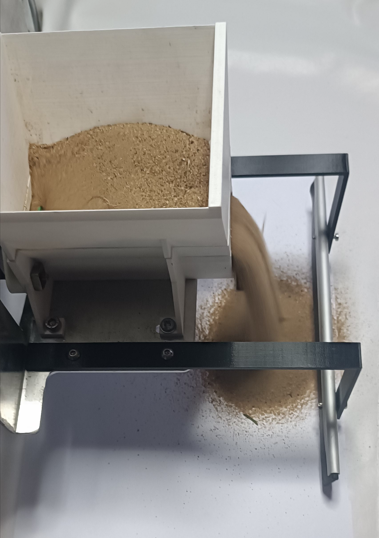
\includegraphics[width=\textwidth]{figures/sand_dispensing.png}
        \caption{Dispenser in operation.}
        \label{fig:dispenser_action}
    \end{subfigure}
    \hfill
    \begin{subfigure}[b]{0.49\textwidth}
        \centering
        \includegraphics[width=\textwidth]{figures/sand_volume.png}
        \caption{Measuring the collected volume.}
        \label{fig:dispensed_volume}
    \end{subfigure}
    \caption[Experimental Setup for the Dispenser Test.]
    {The physical setup for the dispenser flow rate test, showing the dispenser in operation (a) and the subsequent measurement of the collected material (b).}
    \label{fig:dispenser_test}
\end{figure}

The complete experimental data is presented in Table \ref{tab:dispenser_data}. The key finding from this data is the low standard deviation across all test runs, with a maximum of only 6.24 ml. This numerically proves that the dispenser's mechanical output is highly consistent and repeatable.

\begin{table}[h!]
    \centering
    \caption{Experimental data from the dispenser consistency test.}
    \label{tab:dispenser_data}
    \begin{tabular}{c c c c c c}
        \hline
        \textbf{Run Time (s)} & \textbf{Run1 (ml)} & \textbf{Run2 (ml)} & \textbf{Run3 (ml)} & \textbf{Average (ml)} & \textbf{Std Dev (ml)} \\
        \hline
        5                     & 125                & 120                & 125                & 123.3                 & 2.36                  \\
        10                    & 240                & 235                & 245                & 240.0                 & 4.08                  \\
        15                    & 365                & 375                & 370                & 370.0                 & 4.08                  \\
        20                    & 515                & 525                & 530                & 523.3                 & 6.24                  \\
        \hline
    \end{tabular}
\end{table}

This strong linear relationship is visualized in Figure \ref{fig:dispenser_graph}. A linear trendline fitted to the average data points shows an \texttt{R-squared} value of 0.992, which represents a near-perfect correlation between runtime and dispensed volume. Based on this data, the dispenser has a calculated average flow rate of approximately 25.6 ml/second.

\begin{figure}[h!]
    \centering
    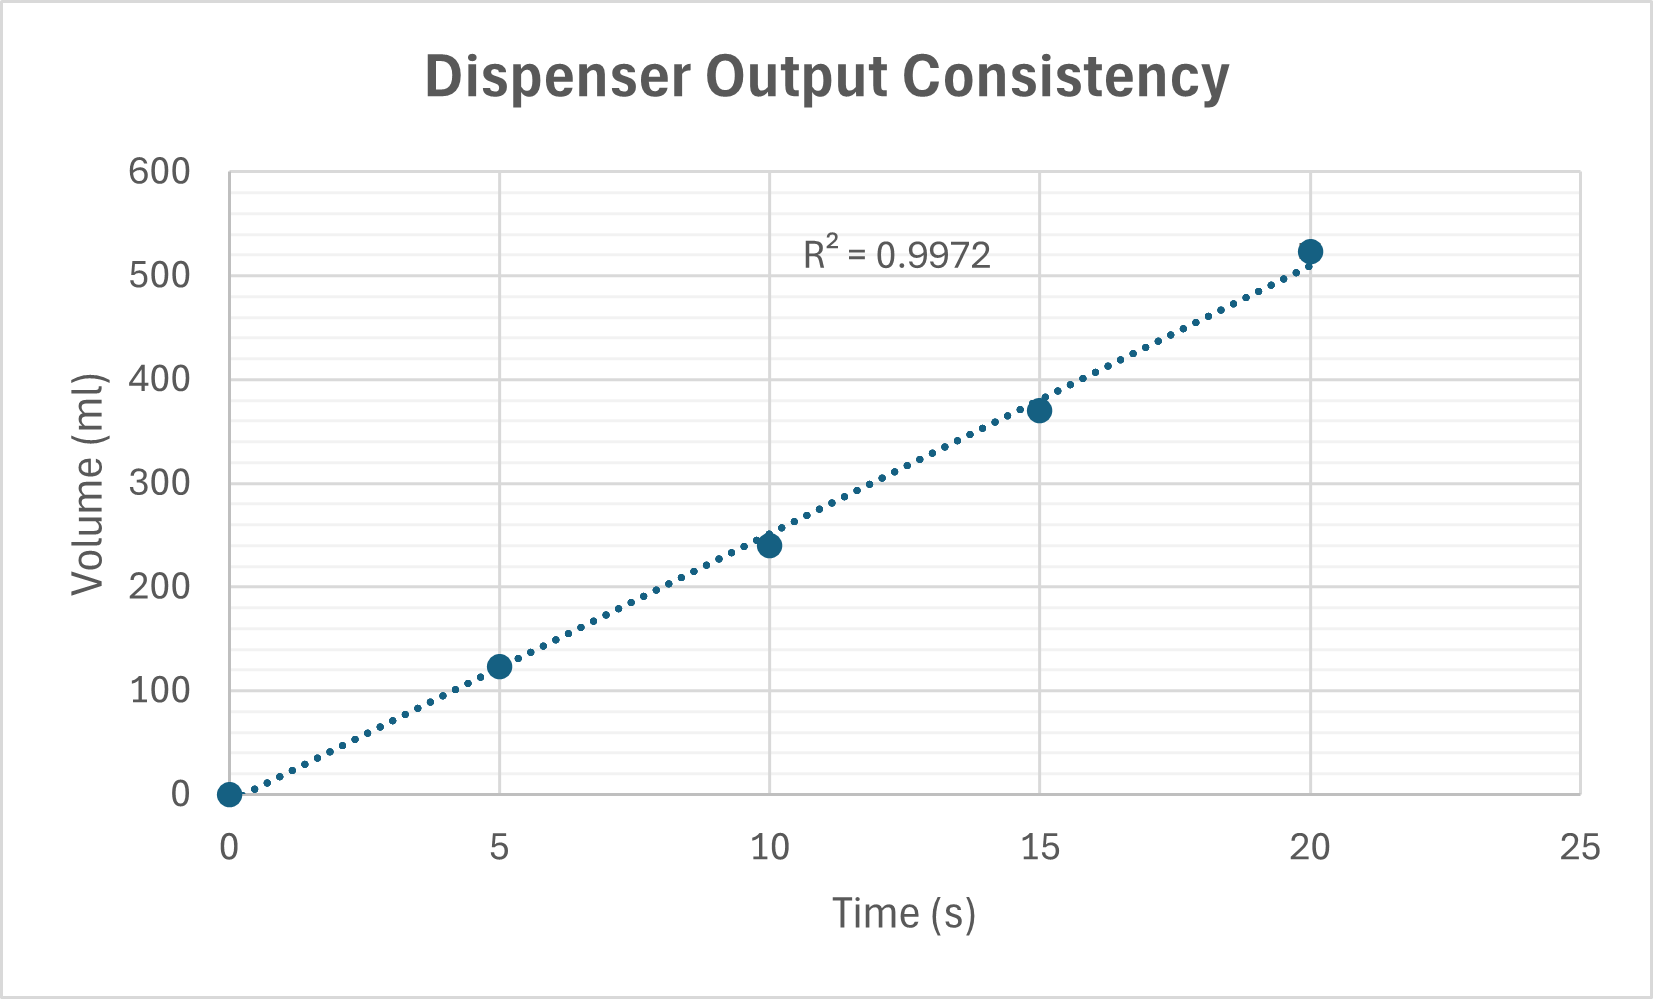
\includegraphics[width=0.8\linewidth]{figures/dispenser_graph.png} % Replace with your final graph's filename
    \caption[Dispenser Output Consistency Graph.]
    {A scatter plot of average dispensed volume versus motor runtime. The data points show a clear linear trend, and the high \texttt{R-squared} value (0.992) of the fitted line confirms the system's high degree of predictability.}
    \label{fig:dispenser_graph}
\end{figure}

The combination of the low standard deviation and the high \texttt{R-squared} value provides strong quantitative evidence that the dispenser is a reliable and precisely controllable mechanism. This validates that the amount of dispensed material can be accurately controlled by varying the motor's run time, making the dispenser a viable and effective component for the final, fully integrated system.

% \section{Mechanical Dispenser Evaluation}
% \label{sec:dispenser_evaluation}
% The final component to be evaluated was the mechanical dispenser, which is responsible for the physical act of repair. The evaluation focused on the consistency and controllability of its output.

% \subsection{Dispensing Consistency and Flow Rate}
% To measure the dispenser's performance, a simple flow rate test was conducted. The hopper was filled with the sand-seed mixture, and the motor was run continuously for a fixed duration of 10 seconds. The dispensed material was collected and its volume was measured. Figure \ref{fig:dispenser_test} illustrates this experimental process and its results.

% \begin{figure}[h!]
%     \centering
%     \begin{subfigure}[b]{0.49\textwidth}
%         \centering
%         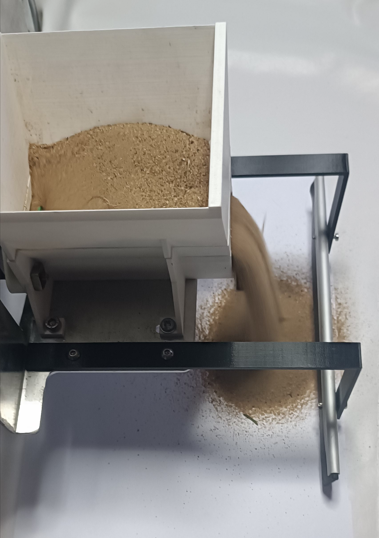
\includegraphics[width=\textwidth]{figures/sand_dispensing.png}
%         \caption{Dispenser in operation.}
%         \label{fig:dispenser_action}
%     \end{subfigure}
%     \hfill
%     \begin{subfigure}[b]{0.49\textwidth}
%         \centering
%         \includegraphics[width=\textwidth]{figures/sand_volume.png}
%         \caption{Measured volume after a 10-second run.}
%         \label{fig:dispensed_volume}
%     \end{subfigure}
%     \caption{The dispenser flow rate test. The dispenser in operation (a) and the resulting material collected in a measuring cup (b), showing a volume of approximately 200 ml.}
%     \label{fig:dispenser_test}
% \end{figure}

% \textbf{Configuration.}
% For this test, the stepper motor was configured using the simplified Arduino firmware, which uses hardcoded parameters for reliability. The motor's maximum speed was set to 2000 steps/second with an acceleration of 2000 steps/second².

% \textbf{Results.}
% The test was repeated multiple times, and the dispenser demonstrated a high level of consistency. In each 10-second run, it dispensed an average of 200 ml of the sand-seed mixture. This is equivalent to 200 cm³, as 1 milliliter is equal to 1 cubic centimeter. This result establishes a consistent flow rate of approximately 20 cm³/second.

% \textbf{Controllability.}
% This consistent flow rate proves that the amount of dispensed material can be controlled simply by varying the motor's run time. For example, to dispense the 110 cm³ required to fill the test box from the volume experiment, the motor would need to be run for approximately 5.5 seconds (110 cm³ / 20 cm³/s).

% While the full closed-loop system—where the robot measures a divot's volume and automatically calculates the required dispensing time—was not completed, this experiment successfully validates that the mechanical dispenser is both consistent and controllable, making it a viable mechanism for the final system.

